%! TeX root = ../Parte2.tex

\section{Messaggi privati}

\begin{myframe}{Criptazione e2e}
  Una normale criptazione cripta i messaggi dal client al server e poi li ricripta del server all'altro client. Il \textbf{server} quindi \textbf{vede i messaggi in chiaro}.

  \medskip\pause
  Nella criptazione end to end il server non può decriptare il messaggio: la chiave è nota solo ai client.
\end{myframe}

\begin{myframe}{WhatsApp}
  \begin{columns}
    \begin{column}{.5\textwidth}
      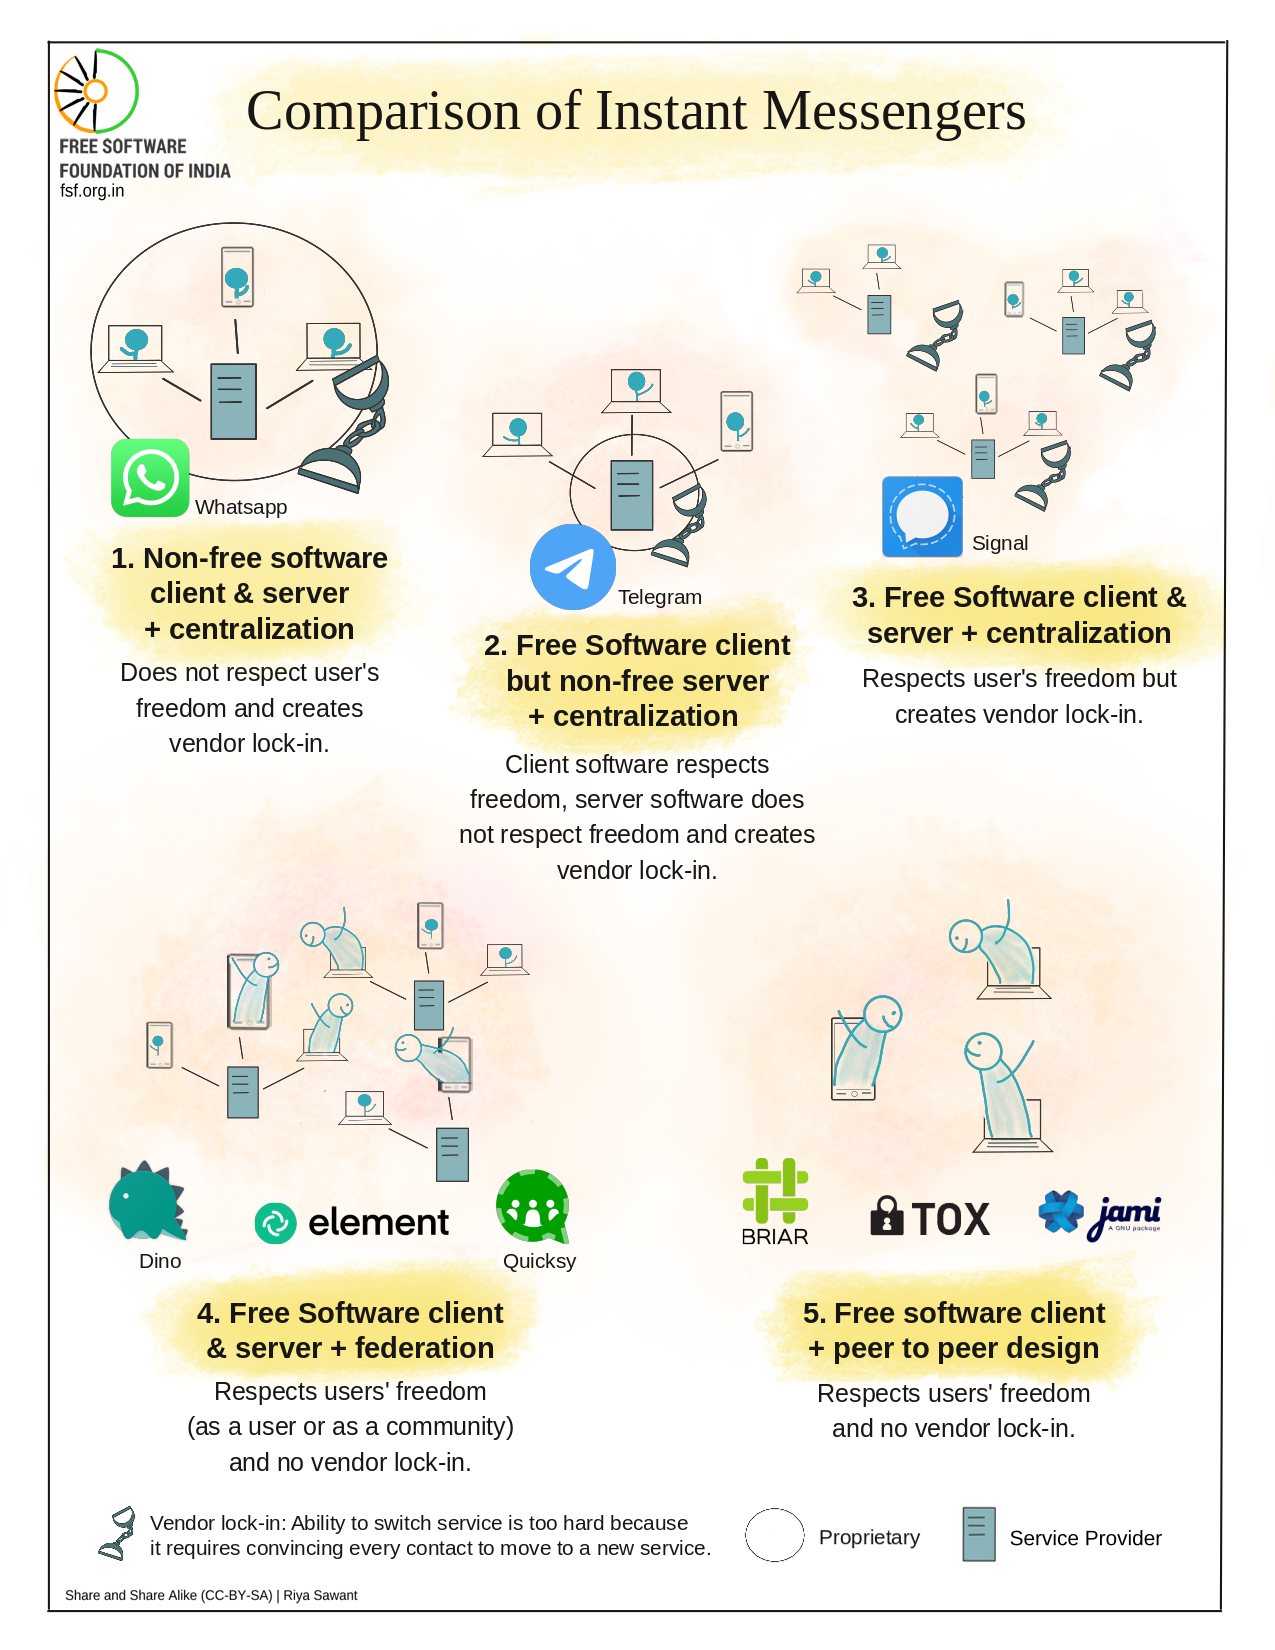
\includegraphics[width=.9\textwidth]{img/chat}
    \end{column}
    \begin{column}{.5\textwidth}
      \begin{itemize}[<+->]
        \item Criptazione e2e;
        \item Backdoor invia chiavi al server: come se non fosse criptata e2e;
        \item Backup non criptato;
        \item Codice proprietario: non sappiamo cosa altro faccia.
      \end{itemize}
    \end{column}
  \end{columns}
\end{myframe}

\begin{myframe}{Telegram}
  \begin{columns}
    \begin{column}{.5\textwidth}
      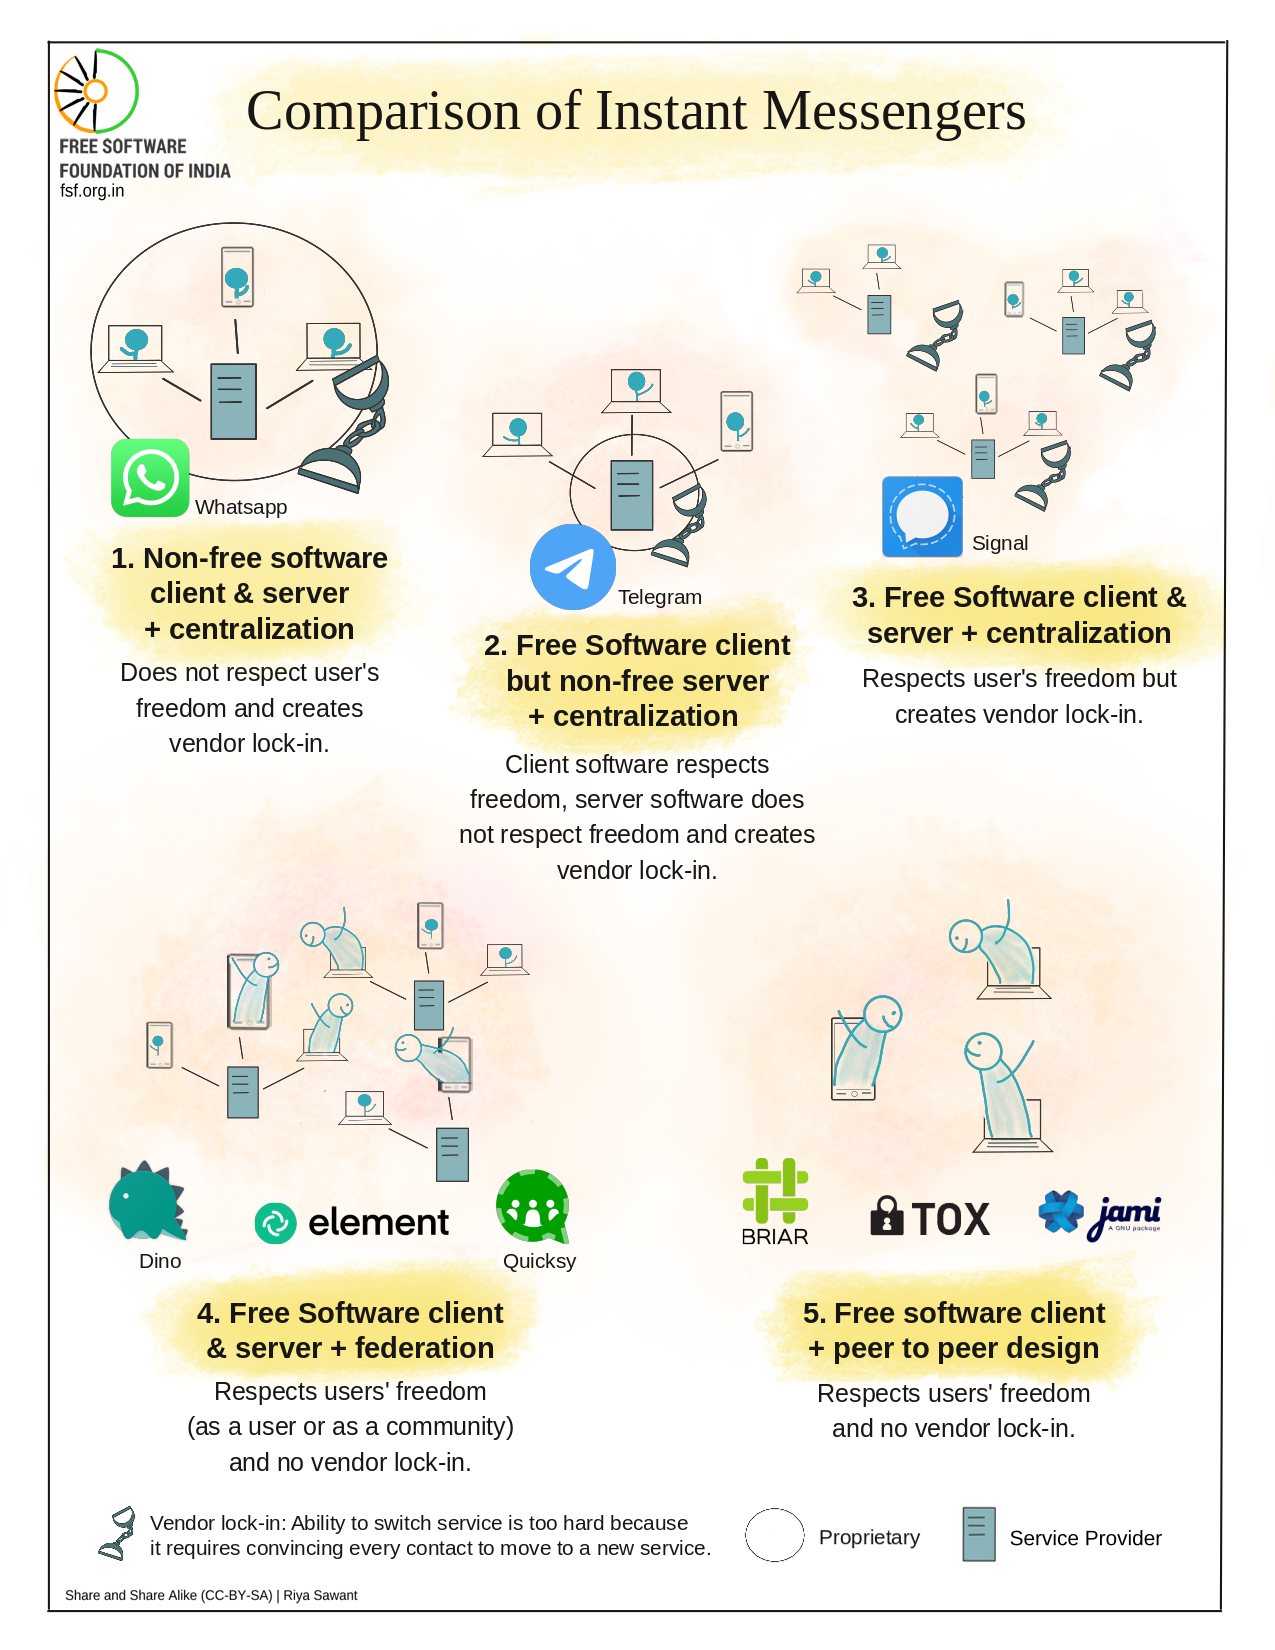
\includegraphics[width=.9\textwidth]{img/chat}
    \end{column}
    \begin{column}{.5\textwidth}
      \begin{itemize}[<+->]
        \item Criptazione e2e solo chat segrete;
        \item I messaggi sono salvati non su un unico server, ma a pezzi su server diversi, in giurisdizioni diverse;
        \item Client è libero (free and open source), server no.
      \end{itemize}
    \end{column}
  \end{columns}
\end{myframe}

\begin{myframe}{Signal}
  \begin{columns}
    \begin{column}{.5\textwidth}
      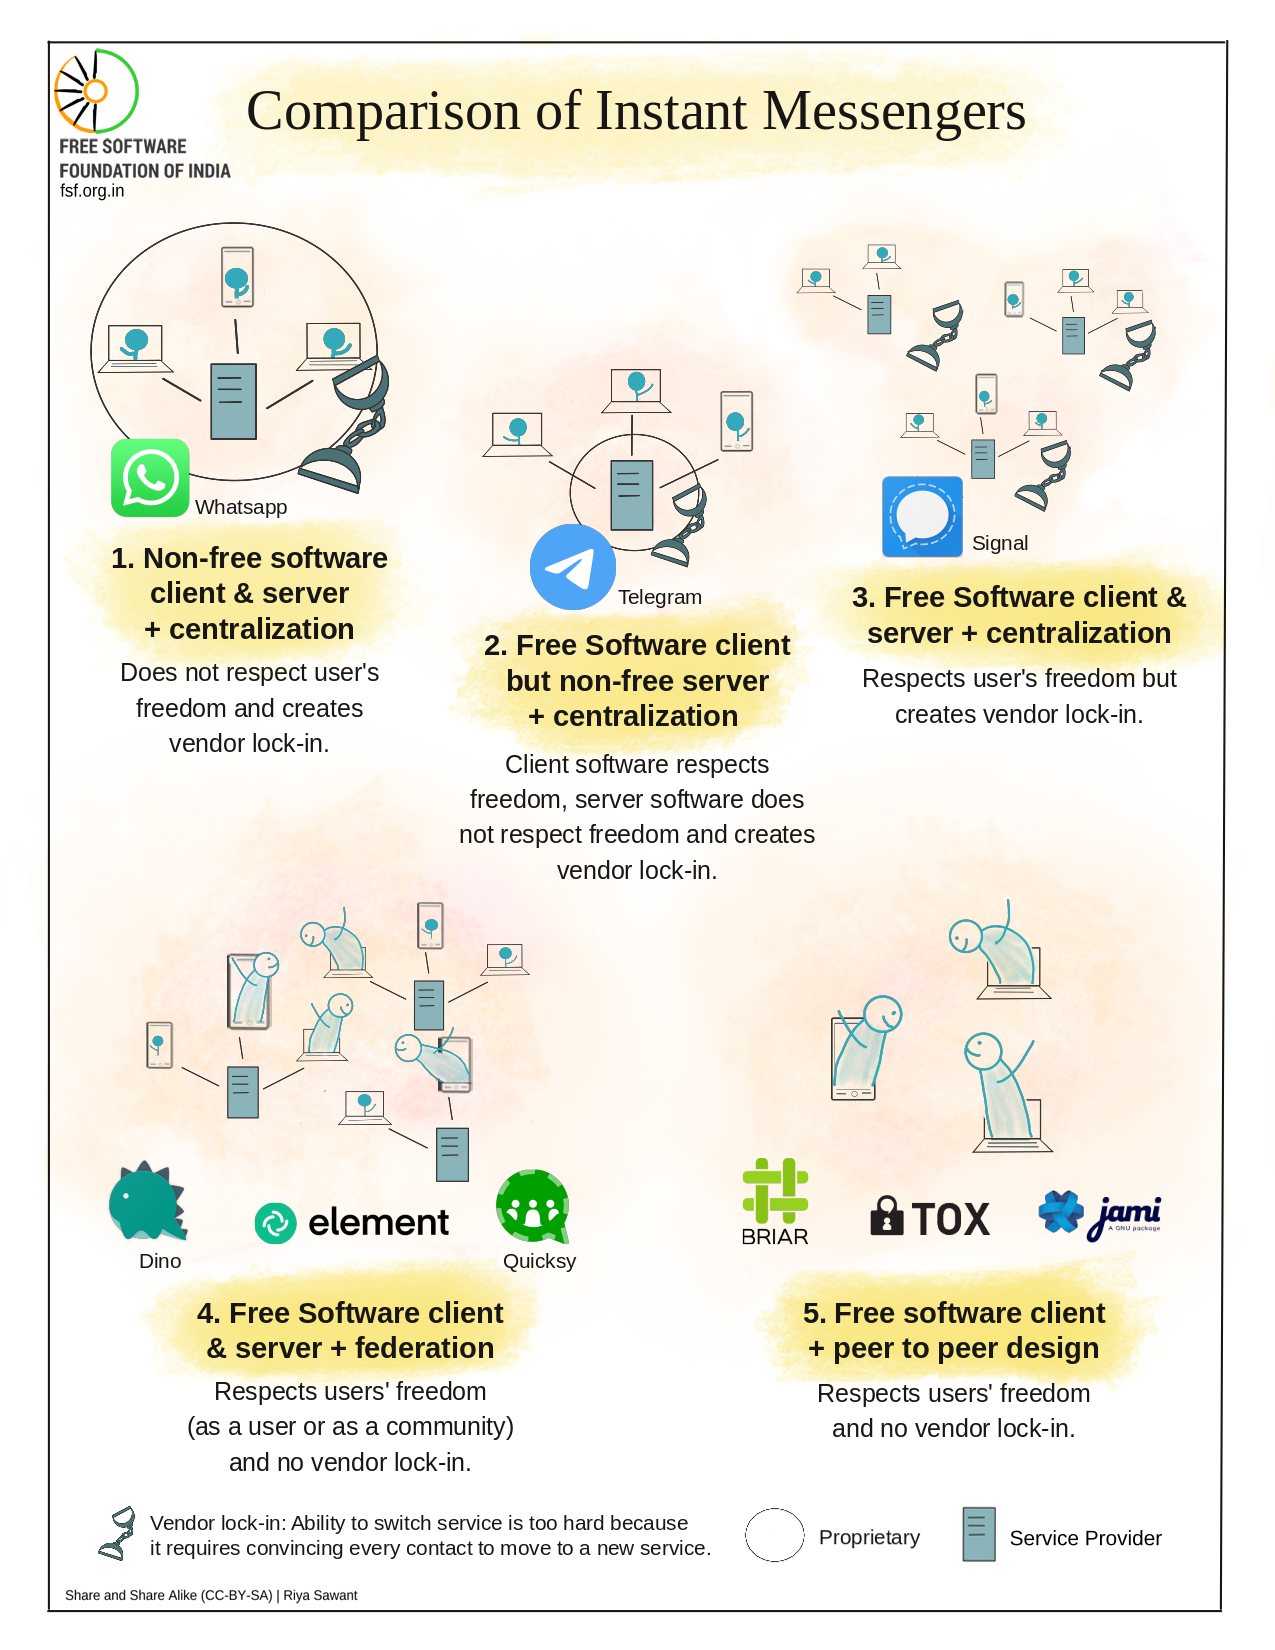
\includegraphics[width=.9\textwidth]{img/chat}
    \end{column}
    \begin{column}{.5\textwidth}
      \begin{itemize}[<+->]
        \item Criptazione e2e;
        \item I messaggi non sono salvati sui server;
        \item Client e server sono liberi;
        \item Server centralizzato.
      \end{itemize}
    \end{column}
  \end{columns}
\end{myframe}

\begin{myframe}{Matrix}
  \begin{columns}
    \begin{column}{.5\textwidth}
      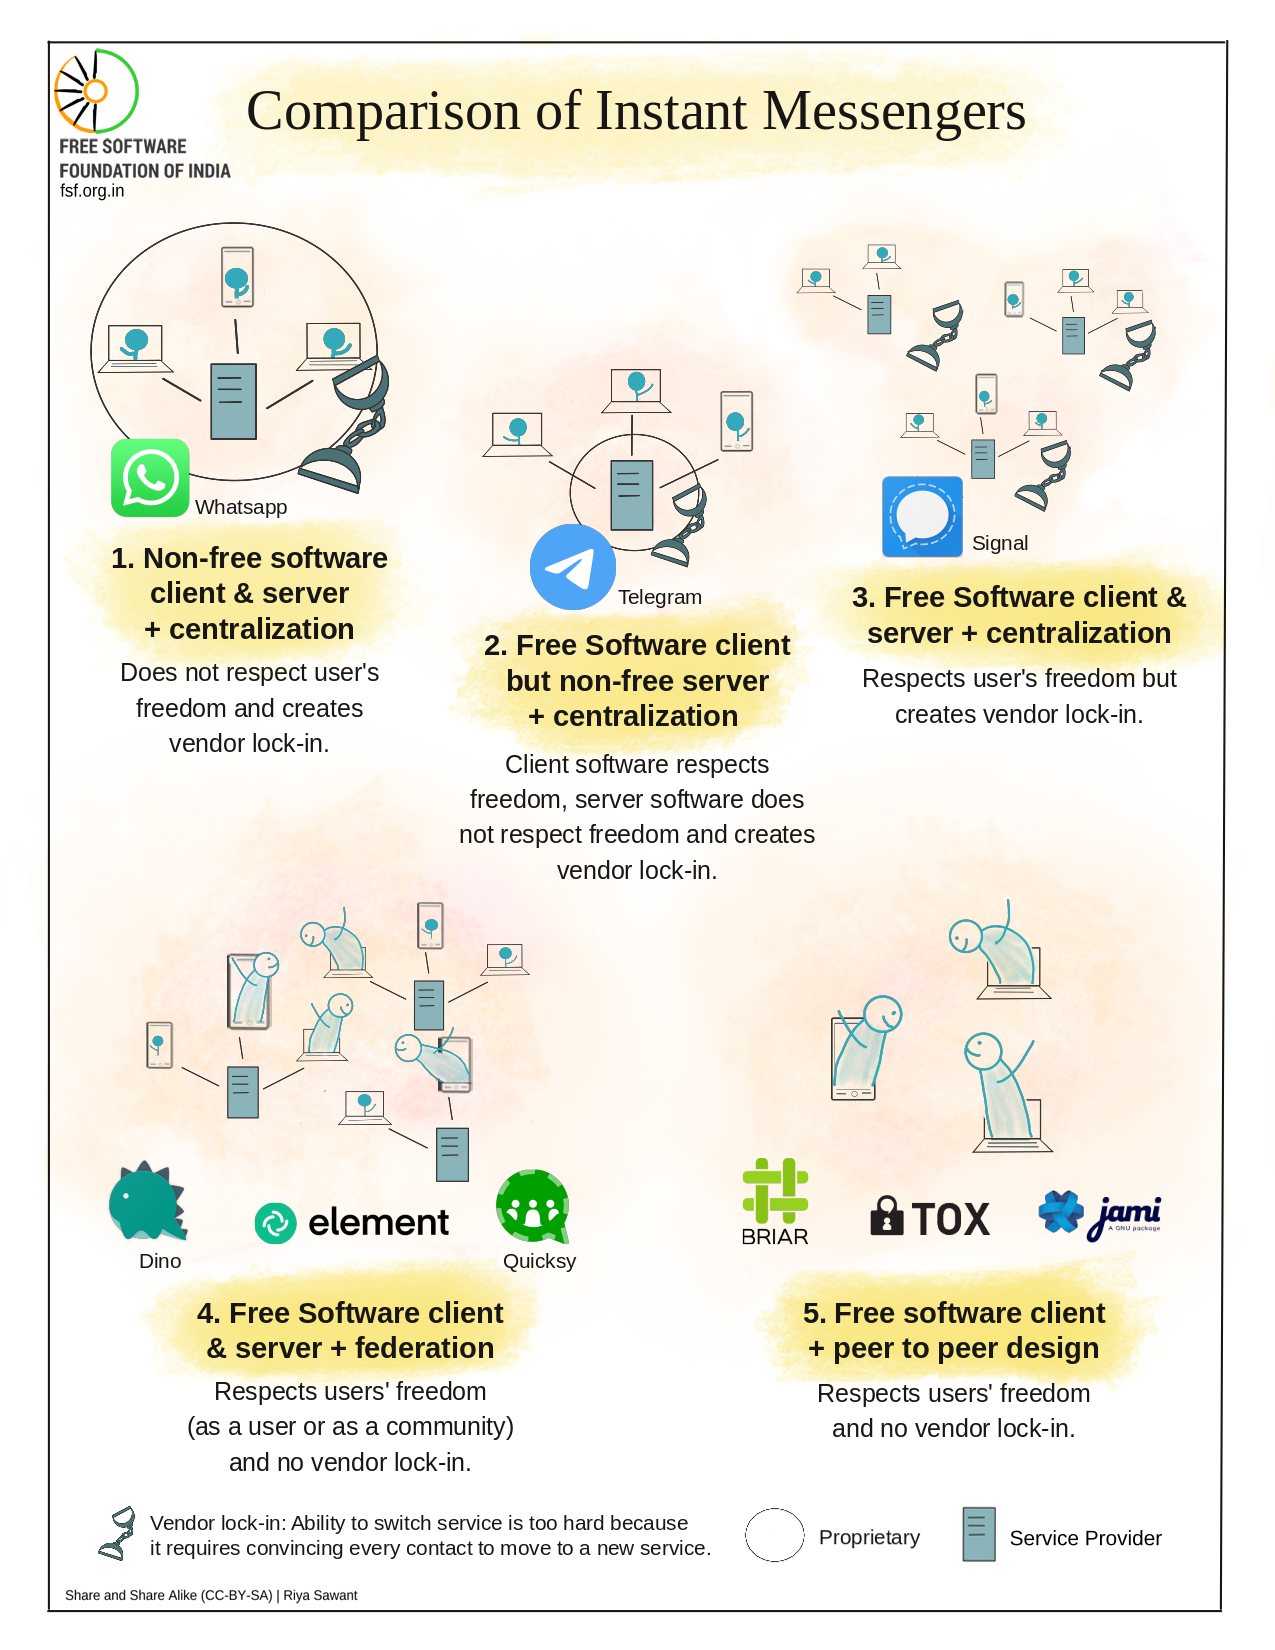
\includegraphics[width=.9\textwidth]{img/chat}
    \end{column}
    \begin{column}{.5\textwidth}
      \begin{itemize}[<+->]
        \item Criptazione e2e;
        \item I messaggi sono salvati sui server, criptati;
        \item Client e server sono liberi;
        \item Server decentralizzati.
      \end{itemize}
    \end{column}
  \end{columns}
\end{myframe}

\begin{myframe}{P2P}
  \begin{columns}
    \begin{column}{.5\textwidth}
      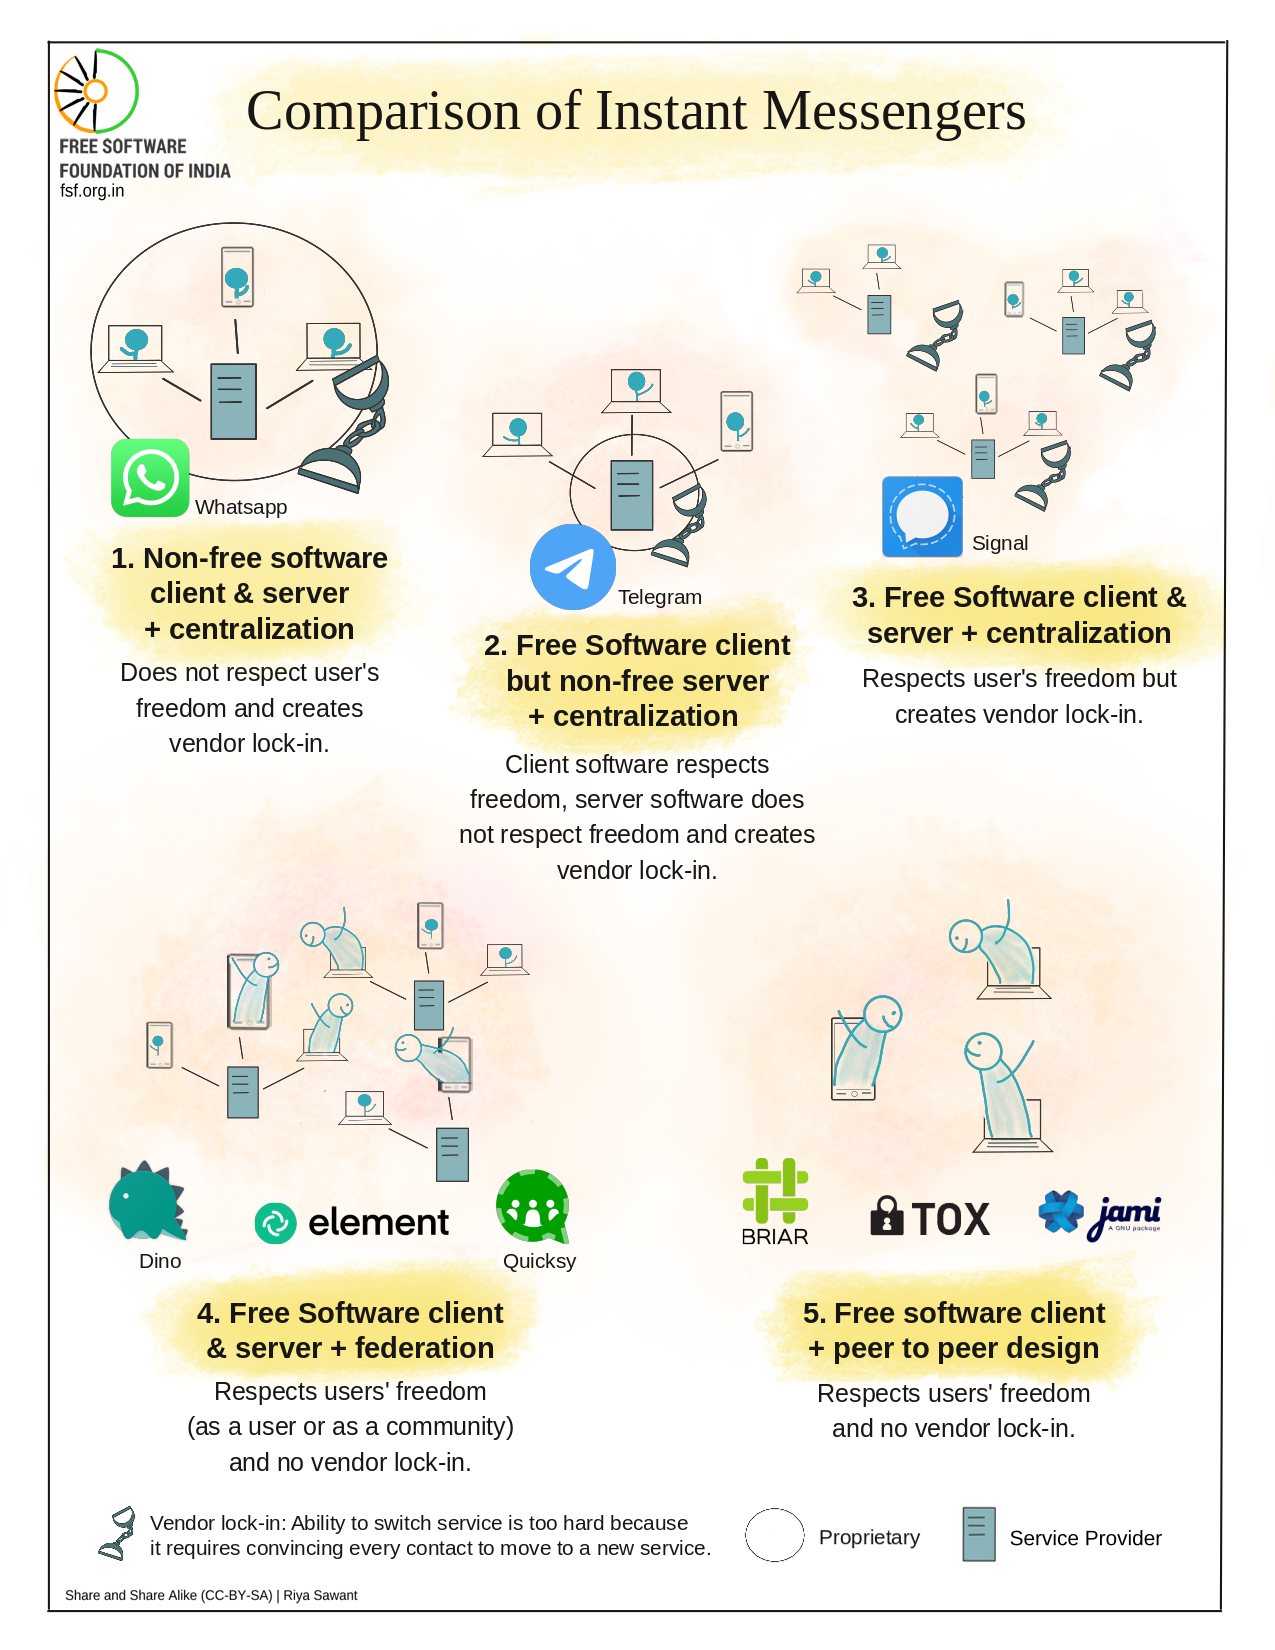
\includegraphics[width=.9\textwidth]{img/chat}
    \end{column}
    \begin{column}{.5\textwidth}
      \begin{itemize}[<+->]
        \item Non esiste il server.
      \end{itemize}
    \end{column}
  \end{columns}
\end{myframe}

\begin{myframe}{Mail}
  Le mail viaggiano sempre in chiaro.

  \medskip\pause
  Esistono servizi di mail criptate (es: Tutanota), ma solo al'interno dello stesso dominio.

  \bigskip\pause
  Si può usare Gnu Privacy Guard (GPG) per criptare il contenuto di una mail (non l'oggetto) a mano.
\end{myframe}


